\chapter{Richtliniendemonstration}

Im Kapitel \ref{sec:analyse-der-aufgabenstellung} im Abschnitt ``\nameref{sec:architekturrichtlinien}'' ging das Projektteam ausführlich auf die in der \nameref{sec:aufgabenstellung} vorgestellten Architekturrichtlinien und Prinzipien ein.

Als Ergebnis dieser Analyse entstand die unter Punkt \ref{sec:how-to-show-principles} vorgestellte, konsolidierte Liste mit Architekturrichtlinien.

Dieses Kapitel soll nun aufzeigen, wie und insbesondere wo eine jeweilige Architekturrichtlinie in der entwickelten Beispielapplikation demonstriert werden konnte.

Dabei wird zuerst verifiziert, ob die potentielle Demonstrationsstelle aus Tabelle \ref{fig:how-to-show-principles-matrix} wie erwartet umgesetzt werden konnte.
Anschliessend wird das konkret zur Richtlinie entstandene Beispiel näher analysiert und erklärt.

Am Ende dieses Kapitel wird bewertet, wie gut die jeweiligen Richtlinien an der Beispielapplikation demonstriert werden konnten.

\section{RP1 REST}
\section{RP2 Application Logic}
\section{RP3 HTTP}
\section{RP4 Link}
\section{RP5 Non Browser}
\section{RP6 Should-Formats}
\section{RP7 Auth}
\section{RP8 Cookies}
\section{RP9 Session}
\section{RP10 Browser-Controls}
\label{sec:principle-rp10-browser-controls}
\begin{quotation}
Man befindet sich auf einem Online-Shop und sucht mit Hilfe der eingebauten Suche Zubehör für seine neu ergatterte Fotokamera. Das Suchresultat ist aber noch zu grob. Deshalb klickt man auf den Zurück-Knopf des Browsers um auf die Suche zurück zu gelangen. Aber was uns hier erwartet, ist nicht etwa das Suchformular, welches man erwartet hätte, sondern die Startseite.
\end{quotation}
Dies ist nicht etwa ein fiktives Beispiel, sondern ein reelles Szenario aus dem Online-Shop des Elektronikgrosshändlers Digitec \cite{Digitec}.

Das ROCA-Prinzip ``Browser-Controls'' will genau dieses unangenehme Erleben verhindern.

\subsection*{Geplante Umsetzung}

``Browser-Controls'' ist sehr eng mit dem Prinzip ``\nameref{sec:principle-rp4-link}'' verbunden. Indem jede Seite ihre eigene \gls{URI} hat und diese beim Navigieren in die ``History'' des Browsers eingefügt wird, funktionieren die Standardbedienelemente (Zurück, Vorwärts und Aktualisieren) eines Browsers erwartungsgemäss.

Dies soll auch in der Beispielanwendung ``Roomies'' der Fall sein. Jeder Seitenwechsel soll über den Webseitenverlauf im Browser nachvollziehbar sein und somit dem Benutzer erlauben, die eingebauten Funktionen des Browsers zu benutzen.

\subsection*{Konkrete Umsetzung}
Mit der Funktion ``Backbone.history.start()'' \cite{BackbonejsHistory} bietet Backbone.js eine Anbindung an die History API \cite{HistoryAPI} an und ermöglicht damit JavaScript Applikationen das dynamische Navigieren inklusive einer Aktualisierung der URL bei Seitenwechseln.

\begin{lstlisting}[language=JavaScript, caption=Activierung der History in Barefoot \cite{BarefootStartClient}, label=lst:barefootStartClientHistory, firstnumber=29]
// from modernizr, MIT | BSD
// http://modernizr.com/
var useHistory = !!(window.history && history.pushState);

Backbone.history.start({
	pushState: useHistory
	, hashChange: useHistory
	, silent: true
});
\end{lstlisting}

\subsection*{Diskussion}
-
\section{RP11 POSH}
\label{sec:principle-rp11-posh}

``POSH'', ausgeschrieben ``Plain Old Semantic HTML'', bezeichnet das Erstellen von HTML-Seiten mithilfe von semantischen Elementen. \cite{SemanticHTML}

Semantisches HTML bietet den Vorteil, dass ``\glspl{SearchEngineSpider}'' die Seite besser verstehen, interpretieren und kategorisieren können. Wird eine Seite gut kategorisiert erscheint sie eher bei einer Suche in einer Suchmaschine wie Google oder Bing.

\subsection*{Geplante Umsetzung}
Die Seiten, respektiv deren HTML Markup, der Anwendung sollen eine klare und logische Struktur beinhalten.
Alle Seiten haben einen Titel, eine Überschrift und Inhalt.
Für Überschriften werden die Tags \emph{h1}, für die grösste und wichtigste Überschrift, bis \emph{h6} für die am wenig wichtigsten.
Tabellen sollen für tabellarische Daten verwendet werden und nicht etwa um die Seite zu strukturieren, wie es in der Vergangenheit oft angewendet wurde.

\subsection*{Konkrete Umsetzung}
Um die möglichen semantischen Inkorrektheiten zu reduzieren, wurde mit Templates gearbeitet. So können beispielsweise Menüs oder Fusszeilen definiert und wiederverwendet werden, ohne dass man diese bei jeder Benutzung neu schreiben muss. Dies geht sehr stark nach dem ``\gls{DRY}'' Prinzip. So werden Fehler verhindert, indem man sie gar nicht zu schreiben hat.

Im folgenden Beispiel-HTML sieht man einen kleinen Ausschnitt aus dem Haupttemplate von ``Roomies''. Man kann klar die Aufteilung der Seite erkennen. Oben beginnter der Header mit dem Menü, gefolgt von einem Platzhalter für allfälligen Fehler-, Warnungs- oder Informationsmeldungen. Die Hauptsektion mit der ID ``main''. Darin Befindet sich die ganzen Inhalte. Und zum Schluss die Fusszeile, in welcher sich der Abmelden-Link befindet.

\begin{lstlisting}[language=HTML, caption=Layout Definition \cite{roomiesHtmlSkeleton}, label=lst:layoutDefinition, firstnumber=27]
<body>
	<header id="menu"></header>
	<div id="flash-messages" class="row flash-messages"></div>
	<section id="main"></section>
	<footer id="footer"></footer>
</body>
\end{lstlisting}

\subsection*{Diskussion}

\section{RP12 Accessibility}
\label{sec:principle-rp12-accessibility}
Aufbauend auf dem Prinzip ``\nameref{sec:principle-rp11-posh}'' besagt das Prinzip \emph{Accessibility}, dass alle Seiten für Hilfesoftware/-geräte wie \emph{Screen Reader} oder \emph{Braillezeile} zugänglich sein müssen.


``Barrierefreiheit schliesst sowohl Menschen mit und ohne Behinderungen als auch Benutzer mit technischen (Textbrowser oder PDA) oder altersbedingten Einschränkungen (Sehschwächen) ... ein.'' \cite{BarrierefreiesInternet}

\emph{RP12 Accessibility} beschränkt sich dabei auf Zugänglichkeit über Hilfeanwendungen. So wird die in der Definition erwähnte Problematik \emph{Farbblindheit} (richtige Farbenwahl etc.) oder die Navigation ohne Maus nicht abgedeckt.

\subsection*{Geplante Umsetzung}
Damit Hilfesoft- und Hilfehardware das User Interface der Beispielapplikation interpretieren kann, soll das HTML Markup, wie unter \ref{sec:principle-rp11-posh} ``\nameref{sec:principle-rp11-posh}'' erklärt, eine semantisch korrekte Struktur aufweisen.

\subsection*{Konkrete Umsetzung}

\emph{Roomies} verwendet, wo nötig, semantisch korrekte HTML-Elemente.

\subsection*{Diskussion}
In ``\nameref{sec:principle-rp11-posh}'' wird ausführlich über die Wichtigkeit eines barrierefreien Internets diskutiert. Das Prinzip \emph{RP12 Accessibility} strebt durch die notwendigen Vorkehrungen in die selbe Richtung, hat aber die Unterstützung gehandicapter Personen zum Ziel.

Leider gehört die Berücksichtigung von Farbenblindheit o.Ä. nicht zum Repertoire von \emph{RP12}. Für das Projektteam gehören aber auch diese Themen klar zum Aufgabenbereich der Richtlinie \emph{Accessibility}.

Das Projektteam schlägt darum die Ergänzung von \emph{RP12 Accessibility} um die erwähnten Punkte vor. Machen es die Anforderung nötig, empfiehlt das Projektteam die Umsetzung von \emph{RP12}.
\section{RP13 Progressive Enhancement}
\label{sec:principle-rp13-progressive-enhancement}

\subsection*{Geplante Umsetzung}


\subsection*{Konkrete Umsetzung}


\subsection*{Diskussion}

\section{RP14 Unobtrusive JavaScript}
\label{sec:principle-rp14-unobtrusive-javascript}

Aktuelle Webapplikationen können grob in zwei Kategorien eingeteilt werden:

\begin{figure}[H]
	\begin{table}[H]
		\tablestyle
		\tablealtcolored
		\begin{tabularx}{\textwidth}{l l X}
			\tableheadcolor
				\tablehead Kategorie &
				\tablehead Beispiel &
				\tablehead Erläuterung
				\tabularnewline
			\tablebody
				Statisch &
				\emph{GitHub} \cite{GitHub} &
				User Interface wird auf dem Server gerendert, JavaScript bringt lediglich dynamisch geladene Inhalte, Effekte oder zusätzliche ``optionale'' Features.
				\tabularnewline

				JavaScript Client &
				\emph{Google Drive} \cite{GoogleDrive} &
				User Interface wird komplett im Browser mittels JavaScript aufgebaut. Ohne JavaScript keine Funktionalität oder schlechtere User Experience.
				\tabularnewline
			\tableend
		\end{tabularx}
	\end{table}
	\caption{Kategorisierung aktueller Webapplikationen}
	\label{tab:current-webapplication-categories}
\end{figure}

Die Kategorie \emph{Statisch} zeichnet sich durch eine hohe Kompatibilität mit allen möglichen Internetbrowsern aus. Durch die Generierung des HTML Markups losgelöst vom schlussendlichen Zielclient, liegt die ganze Verantwortung, vom beschaffen anzuzeigender Daten bis hin zum zusammenstellen des HTML \gls{DOM}'s komplett bei der Serverkomponente.

Zwar kommt auch bei diesem Typus oftmals JavaScript zur Anwendung, meist beschränkt sich dessen Anwendung aber auf die Ergänzung des bereits statisch geladenen Inhaltes. So lädt \emph{Mila} \cite{Mila} beim Seitenwechsel, sofern JavaScript aktiviert, neuen Inhalt über einen \gls{AJAX} Request. Nach Erhalt des vorgerenderten HTML Markups aus der Antwort ersetzt es entsprechende Inhalte im aktuell angezeigten HTML \gls{DOM} des Browsers.

Als Programmiersprache auf dem Applikationsserver kommt hier oft Java, Python, PHP, Ruby o.Ä. zum Einsatz.

Beim puren \emph{JavaScript Client} liegt der Programmcode für das Rendern des User Interfaces mit all seinen Inhalten als JavaScript Quelltext vor. Nach erfolgreicher Übertragung zum Internetbrowser initiiert dieser die Erstellung der Applikationsoberfläche im HTML \gls{DOM} des Clients.

Sollen dynamische Informationen angezeigt werden, müssen diese über eine Serviceschnittstelle beim entsprechenden Anbieter angefragt werden (siehe bspw. Abschnitt \ref{sec:principle-rp1-rest} ``\nameref{sec:principle-rp1-rest}'').

Die Verlagerung des User Interface Quelltexts direkt in den Browser hat den Vorteil, dass UI Elemente effizienter verändert und aktualisiert werden können. Soll bspw. nur ein kleiner Teil der Benutzeroberfläche aktualisiert werden, kann dies gezielt und ohne Umweg über einen erneuten Request an den Server geschehen.

Durch diese Vereinfachung entfallen unnötige Wartezeiten zwischen Benutzereingabe und Systemreaktion. Dies resultiert wiederum in einer verbesserten User Experience.

Es ist bereits zu erahnen, dass diese Art von Webapplikation ohne JavaScript-Unterstützung im Browser nicht ausgeführt werden kann. Ein Beispiel hierfür liefert der \emph{Google Drive} \cite{GoogleDrive} Webclient. Wie in Abbildung \ref{fig:googleDriveNoJs} ersichtlich verweigert dieser ohne aktiviertes JavaScript die Funktion und zeigt ein leeres Standardlayout mit einer entsprechenden Meldung an.

\begin{figure}[H]
	\centering
	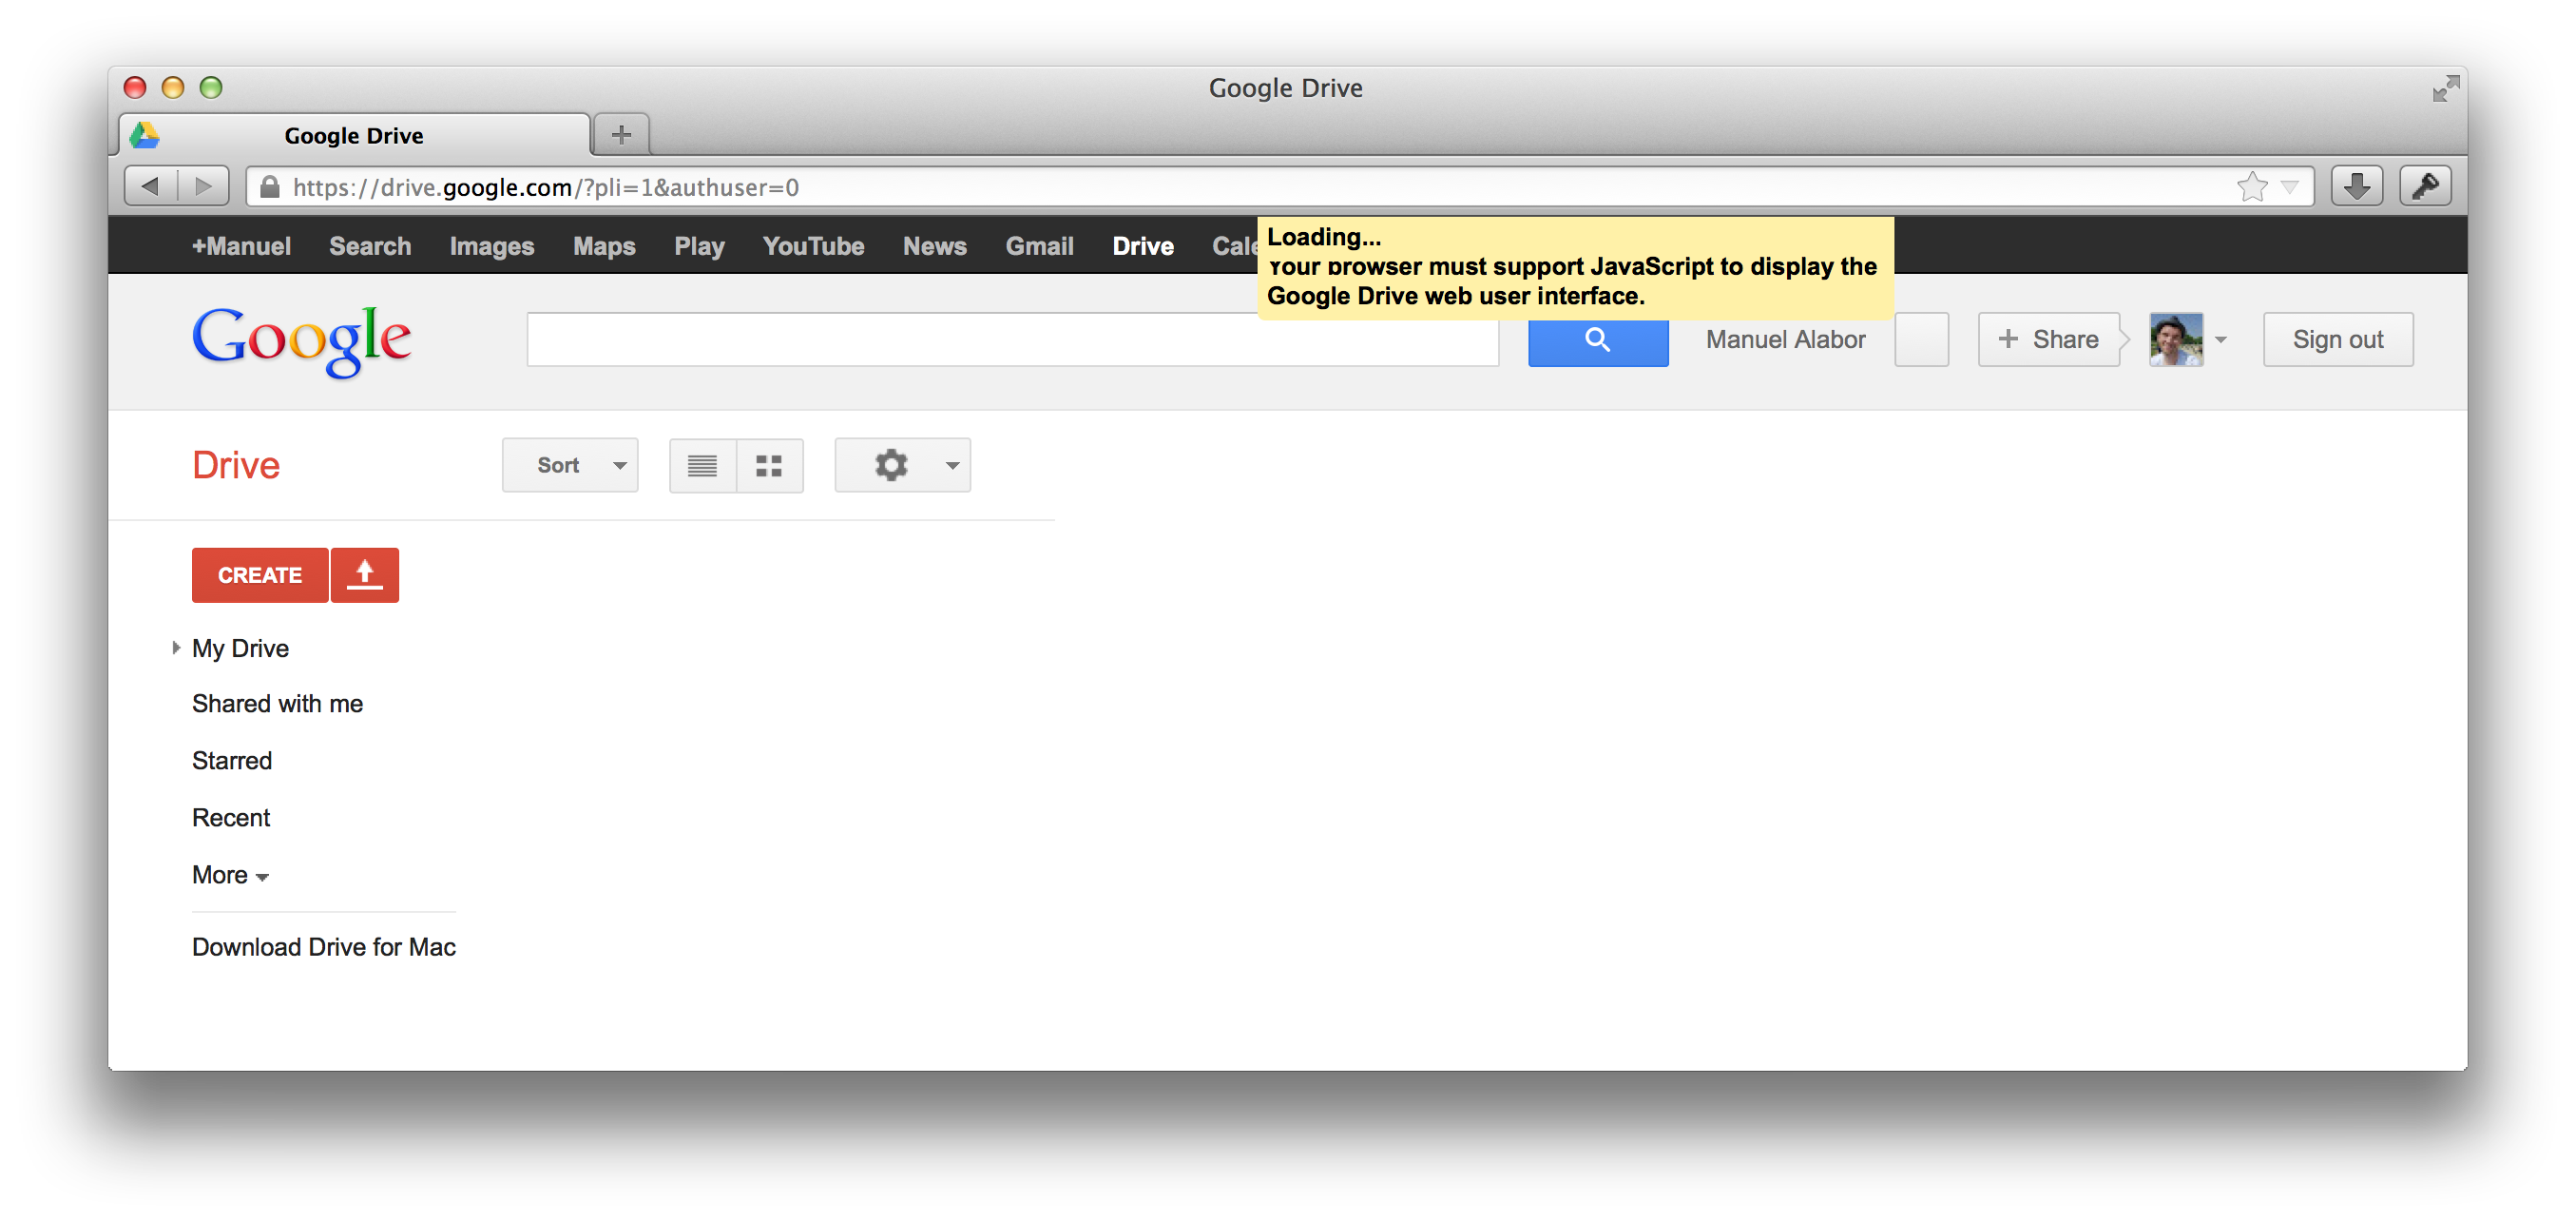
\includegraphics[width=12cm]{content/principle-demonstration/images/googledrive-nojs.png}
	\caption{\emph{Google Drive} in Firefox 21.0 mit deaktiviertem JavaScript}
	\label{fig:googleDriveNoJs}
\end{figure}

Die Richtlinie \emph{RP14 Unobtrusive JavaScript} aus dem ROCA Manifest verlangt, dass eine Webapplikation auch bei deaktiviertem JavaScript weiter funktionstüchtig bleibt. Soll JavaScript für ein modernes User Interface verwendet werden, muss gem. \emph{RP14} also eine Mischform aus den vorgestellten Applikationstypen verwendet werden.
\newline\newline
Bezieht man \emph{Unobtrusive Javascript} neben dem ``Wie und Wo'' User Interfaces gerendert werden auf die Thematik \emph{Codequalität}, gehört ein weiterer Aspekt zu diesem Bereich: Die Vermischung von HTML Markup und JavaScript Code soll unterbunden werden. Hierzu zeigt der Quelltext \ref{lst:badHtmlMarkupWithJavaScript} ein Beispiel, wie es unter keinen Umständen umgesetzt werden sollte.

\begin{lstlisting}[language=HTML, caption={Beispiel einer Vermischung von HTML Markup und JavaScript}, label={lst:badHtmlMarkupWithJavaScript}]
<a href="adresses.html" onClick="$('#progressIndicator').removeClass('hidden');showAddresses();return false;">
	Display Addresses
</a>
\end{lstlisting}

In den Quelltexten \ref{lst:goodHtmlMarkupWithoutJS} und \ref{lst:goodJSOutsideHtmlMarkup} ist ersichtlich, wie eine Separierung von JavaScript Logik und HTML Markup optimal implementiert wird.

\begin{lstlisting}[language=HTML, caption={Beispiel eines sauberen HTML Markups ohne JavaScript}, label={lst:goodHtmlMarkupWithoutJS}]
<a href="adresses.html" id="showAddresses">Display Addresses</a>
\end{lstlisting}

\begin{lstlisting}[language=JavaScript, caption={Beispiel Event-Handler in ausgelagerter JavaScript Datei}, label={lst:goodJSOutsideHtmlMarkup}]
$(function() {
	$('#showAddresses', showAddresses);

	function showAddresses(evt) {
		$('#progressIndicator').removeClass('hidden');
		// ... show addresses
		return false;
	}
});
\end{lstlisting}


\subsection*{Geplante Umsetzung}

Als Herausforderung hat das Projektteam geplant, die Beispielapplikation \emph{Roomies} als Mischung der vorgestellten Applikationstypen umzusetzen.

Grundsätzlich sollen Inhalte statisch auf der Backendkomponente gerendert werden. Hat der Benutzer in seinem Browser JavaScript aktiviert, ermöglicht entsprechender Programmcode die Umsetzung der im einleitenden Abschnitt vorgestellten Funktionalitäten eines vollwertigen \emph{JavaScript Clients}.

Zugriffe auf persistente Applikationsdaten sollen wie in \ref{sec:principle-rp1-rest} ``\nameref{sec:principle-rp1-rest}'' vorgeschlagen in ein entkoppeltes Serviceinterface gekapselt werden.

Um die Wartbarkeit der Codebasis zu optimieren, soll die Separierung von HTML Markup und JavaScript wie beschrieben strikt eingehalten werden.


\subsection*{Konkrete Umsetzung}

Während der Implementation der geplanten Lösung wurde sehr schnell klar, dass die entstehende Applikation zwar wie erwartet die gewünschte hybride Form aufweisen wird, aber keinesfalls mit der ROCA Richtlinie \emph{\nameref{sec:principle-rp15-no-duplication}} vereinbar sein wird.

Es hätten viele Codefragmente wie die View-Templates (Beispiel siehe Quelltext \ref{lst:reusableHandlebarsViewTemplate}) dank der durchgängigen Verwendung von JavaScript auch im Frontend wiederverwendet werden können. Andere, logikintensivere Komponenten wie die Controller zur Steuerung der eigentlichen User Interface Funktionalitäten (Event-Handling, Datenzugriffe etc.) hätten doppelt implementiert werden müssen.

\begin{lstlisting}[language=JavaScript, firstnumber=31, caption={Ausschnitt aus dem \emph{Handlebars} \cite{Handlebars} Template zur Darstellung von Benutzerinformation in der Menüleiste von \emph{Roomies} \cite{roomiesMenuTemplate}}, label={lst:reusableHandlebarsViewTemplate}]
{{#if user}}
<ul class="right">
	<li class="account">
		<a href="/resident/{{user.facebookId}}/profile">
			<span class="item-label">{{user.name}}</span>
			<img class="avatar small" src="//graph.facebook.com/{{user.facebookId}}/picture" />
		</a>
	</li>
</ul>
{{/if}}
\end{lstlisting}

Um diesem Umstand gegensteuern zu können teilte sich das Projektteam nach der ersten Entwicklungsiteration in zwei Gruppen:

\begin{itemize}
	\item Zwei Mitglieder arbeiteten weiter an der Umsetzung der geplanten Use Cases
	\item Ein Mitglied fokussierte sich auf die Entwicklung einer Möglichkeit, identischen Applikationscode sowohl in der Backend-Komponente für statisches Rendering als auch direkt im Browser als JavaScript Client verwenden zu können.
\end{itemize}

Aus diesem Prozess entstand das eigenständige Framework \emph{barefoot} \cite{Barefoot}. Es setzt auf der verbreiteten Bibliothek \emph{Backbone.js} \cite{Backbonejs} auf und ermöglicht die Verwendung einer einzigen, einheitlichen Codebasis für JavaScript-basierte Webapplikationen (siehe dazu auch Kapitel ``\nameref{sec:sad}'' Abschnitt \ref{sec:sad-implementation}).

Mit der Integration des neuartigen Frameworks kann, ähnlich wie bei \emph{rendr} \cite{rendr}, jedoch ohne \emph{CoffeeScript}, komplett auf doppelte Codefragmente verzichtet werden. Gleichzeitig profitiert der Endbenutzer von kurzen Lade- und Reaktionszeiten im User Interface. Sollte auf dem Client kein JavaScript verfügbar sein, greift automatisch das klassische servergestützte Rendering und alle Funktionalitäten bleiben zugänglich.

\subsection*{Diskussion}

Ähnlich den zwei Typen von Webapplikationen sind zwei kontroverse Strömungen in der Entwicklergemeinschaft erkennbar \cite{StackOverflowUnobtrusiveJavascriptOutdated}: Die eine Gruppe drängt zur alleinigen Nutzung der neusten Features und tendiert daher eher zu Lösungen mit reinen \emph{JavaScript Clients}. Andere Gruppierungen geben sich vergleichsweise konservativ. Sie argumentieren damit, dass:

\begin{itemize}
	\item zum Einen die Kompatibilität zu weniger leistungsstarken Browsern resp. JavaScript Engines (Smartphones, alte Browserversionen etc.) gewährleistet sein muss
	\item zum anderen die Umsetzung einer eben solchen \emph{unobtrusive} Lösung entsprechend aufwändig sei.
\end{itemize}

Beiden Lagern kann das Projektteam mit der umgesetzten Beispielapplikation entgegentreten: Mit \emph{barefoot} sind Webapplikationen möglich, welche mit einer einzigen, durchgängigen Codebasis sowohl das statische als auch clientseitige Rendering von User Interfaces resp. deren Ausführung ermöglicht. Daraus resultiert eine im Vergleich zur doppelten Implementierung höhere Effektivität im Entwicklungsprozess. Gleichzeitig kann das Erlebnis für den Endbenutzer optimiert werden.

Ob sich die Investition in die Entwicklung einer Webapplikation, welche \emph{RP14 Unobtrusive JavaScript} genügt, lohnt, kann das Projektteam nicht pauschal beantworten. Je nach Anforderungen kann die Erfüllung dieser Richtlinie aber zu einer höheren Akzeptanz bei den Benutzern führen. Frameworks wie \emph{barefoot} können zudem künftig dazu beitragen, einfacher eine ``unobtrusive'' Lösung umzusetzen.

\section{RP15 No Duplication}
\label{sec:principle-rp15-no-duplication}

Um \emph{RP15} einfach erklären zu können, soll folgendes Beispiel dienen:

\begin{quotation}
In einer Webapplikation sollen die Benutzereingaben aus einem Formular auf formale Korrektheit hin geprüft werden. Beim Versenden des Formulars werden dazu die übertragenen Informationen in der Backendkomponente überprüft und ggf. mit einer Fehlermeldung zurückgewiesen.

Für eine Verbesserung der User Experience soll nun bereits vor dem Versenden des Formulars im Frontend eine Prüfung der Eingaben gemacht werden. Da die Backendkomponente mit PHP implementiert wurde, entscheidet der zuständige Entwickler den bestehenden Code mit JavaScript auf den Client zu portieren.
\end{quotation}

Das Beispiel verdeutlicht, welche Stellen einer Webapplikation tendenziell besonders anfällig für duplizierten Quelltext sein können.

Die Richtlinie 15 \emph{No Duplication} soll die Erstellung von doppelten Codefragmenten minimieren resp. komplett verhindern.


\subsection*{Geplante Umsetzung}

Die Aufhebung der Sprachbarriere, welche durch Verwendung von JavaScript sowohl auf Client- als auch auf Serverseite resultiert, soll bereits zu einem grossen Teil zur Vermeidung von doppelten Codefragmenten beitragen.

Das Projektteam will zudem durch geschickte Erstellung von Modulen die Wiederverwendbarkeit des enthaltenen Quelltexts erleichtern.


\subsection*{Konkrete Umsetzung}

Mit der durchgängigen Verwendung von \emph{barefoot} \cite{Barefoot} für die Implementation der Beispielapplikation konnte der Anspruch von \emph{RP15 No Duplication} besser als erwartet umgesetzt werden.

Wie unter ``Konkrete Umsetzung'' im Abschnitt \ref{sec:principle-rp14-unobtrusive-javascript} ``\nameref{sec:principle-rp14-unobtrusive-javascript}'' bereits ausführlich beschrieben wurde, konnte eine durchgängige und duplikatfreie Codebasis umgesetzt werden.


\subsection*{Diskussion}

Unabhängig von der Entwicklung von Webapplikationen kennt der Software Engineer das Prinzip von \emph{Don't repeat yourself}. Dementsprechend bietet \emph{RP15 No Duplication} eigentlich keine grundlegenden Neuerungen. Wie in der Beispielapplikation aufgezeigt werden konnte, erleichtert die Verwendung der gleichen Programmiersprache in Front- und Backend die Umsetzung von \emph{RP15} zudem zusätzlich.

Lassen es daher die Umstände zu, empfiehlt das Projektteam aufgrund des besser wartbaren Codes die Umsetzung von \emph{RP15 No Duplication} uneingeschränkt.
\section{RP16 Know Structure}
\label{sec:principle-rp16-know-structure}

Gehen wir exemplarisch von einer modernen, entkoppelten Applikationsarchitektur aus, welche eine klare Trennung zwischen Front- und Backend vorsieht, so übernimmt der Frontendteil die Erzeugung des User Interfaces auf dem Clientrechner (Beispiele u.A. bei \emph{TodoMVC} \cite{TodoMVC}).

Das Backend liefert beim initialen Request ein HTML Grundgerüst, auf welchem die JavaScript Logik des Frontends das finale UI aufbaut.

\begin{lstlisting}[language=HTML, caption={Beispiel eines HTML Gerüsts zum Rendering eines User Interfaces}, label=lst:htmlSkeleton, escapeinside={@}{@}]
<html>
<head>
	<meta charset="utf-8">
	<title>HTML 5 Example App - Client Side UI Logic</title>
	<link href="/stylesheets/app.css" rel="stylesheet">
</head>
<body>
	@\label{lst:htmlSkeleton_maindiv}@<div id="main"></div>
	@\label{lst:htmlSkeleton_appjs}@<script src="/javascripts/app.js"></script>
</body>
</html>
\end{lstlisting}

Zeile \autoref{lst:htmlSkeleton_appjs} im Quelltext \ref{lst:htmlSkeleton} zeigt beispielhaft die Einbindung der JavaScript-Datei aus Quelltext \ref{lst:htmlSkeletonJavascriptFile}. Nach Beendigung des Ladevorgangs wird unter Verwendung des \gls{DOM}-Manipulators \emph{jQuery} \cite{jQuery} dynamisch ein Titel-Element in das \emph{<div>}-Element mit der ID \emph{main} eingefügt.

\begin{lstlisting}[language=JavaScript, caption={JavaScript-Datei \emph{app.js} zu Quelltext \ref{lst:htmlSkeleton}}, label=lst:htmlSkeletonJavascriptFile]
$(function() {
	$('div#main').html('<h1>Hello World</h1>');
});
\end{lstlisting}

Das ROCA Prinzip 17 \emph{Know Structure} beschreibt den oben aufgezeigten Aufbau und erachtet es als wichtig, dass die Backendkomponente keine Kenntnis über das vom Frontendteil gerenderten User Interface hat. Das Backend soll lediglich die initiale Struktur des Grundgerüsts aus Quelltext \ref{lst:htmlSkeleton} kennen und später nur noch als Datenlieferant via einer API dienen.


\subsection*{Geplante Umsetzung}

Unter Berücksichtigung des Prinzips \emph{\nameref{sec:principle-rp14-unobtrusive-javascript}}, näher beschrieben im Abschnitt \ref{sec:principle-rp14-unobtrusive-javascript}, wird nicht geplant \emph{RP16 Know Structure} in seiner essentiellen Form innerhalb der Beispielapplikation \emph{Roomies} zur Anwendung zu bringen.


\subsection*{Konkrete Umsetzung}

Wie in Abschnitt \ref{sec:principle-rp14-unobtrusive-javascript} dokumentiert, wurde dem ROCA Prinzip \emph{\nameref{sec:principle-rp14-unobtrusive-javascript}} eine grössere Gewichtung zugestanden als \emph{Know Structure}. Aus diesem Grund wurde wie geplant darauf verzichtet User Interface Logik nur in der Frontendkomponente zu verwenden.

Die aus den Abschnitten \ref{sec:principle-rp15-no-duplication} und \ref{sec:principle-rp14-unobtrusive-javascript} bekannte geteilte Codebasis zwischen Front- und Backendkomponente zielt sogar absichtlich darauf ab, dass auch im Backend die komplette Struktur des User Interfaces bekannt ist.

Ein grundlegender Punkt wurde jedoch aus \emph{RP16 Know Structure} adaptiert: \emph{Roomies} verwendet wie vorgeschlagen ein HTML Grundgerüst \cite{roomiesHtmlSkeleton}, in welches sowohl im Front- als auch Backend die UI Elemente gerendert werden.


\subsection*{Diskussion}

\emph{Separation of concerns} \cite{SeparationOfConcerns} gehört nicht umsonst zu einem der grundlegendsten Prinzipien im Software Engineering. Darauf bezogen hat die eigentliche Intension von \emph{RP16 Know Structure} durchaus seine Daseinsberechtigung: Eine klare Auftrennung von UI Rendering und eigentlicher Geschäftslogik ist erstrebenswert.

Möchte man die Architekturrichtlinie \emph{\nameref{sec:principle-rp14-unobtrusive-javascript}} zwecks bestmöglicher Kompatibilität in die Entwicklung einer Applikation mit einfliessen lassen, kommt es unweigerlich zum Konflikt mit \emph{RP16}. Damit die Applikation auch ohne das User Interface Rendering direkt auf dem Client funktionieren kann, muss die Backendkomponente zwingend über Renderingfunktionalität und damit Wissen über die Struktur des resultierenden HTML Markups verfügen. Damit bricht dieses Vorgehen klar mit den Anforderungen von \emph{Know Structure}.

Kann auf \emph{\nameref{sec:principle-rp14-unobtrusive-javascript}} verzichtet werden, mag \emph{RP16 Know Structure} seine Stärken ausspielen können. Ist jedoch das clientunabhängige Rendering des User Interfaces eine Anforderung an die zu erstellende Lösung, empfiehlt das Projektteam von \emph{RP16} abzusehen.

\section{RP17 Static Assets}
\subsection*{Geplante Umsetzung}
Die ``Static Assets'' ROCA Richtlinie will dass jeglicher JavaScript Code oder CSS Stylesheets für den Client von statischer Natur ist. Dies bedeuted, dass der Server keine dynamische Generierung von diesem Code vornimmt.



\subsection*{Konkrete Umsetzung}
\subsubsection*{CSS Stylesheets}


\subsubsection*{Clientside JavaScript}


\section{RP17 History API}
\section{TP3 Eat your own API dog food}
\section{TP4 Separate user identity and sign-up (...)}
\section{TP7 Apply the Web instead of working around}
\section{TP8 Automate everything or you will be hurt}

%\section{Abschliessende Bewertung}

todo